% !TeX spellcheck = en_US
% !TeX encoding = UTF-8
\section{Metadynamics\label{Sec:ES:metadynamics}}
Metadynamics, vividly called flooding method, was first suggested by Laio and Parrinello in 2002.\cite{LaioPNAS2002} 
%Imaging you became Doraemon in a dream. 
Imaging you were standing in a valley and were surrounded by high mountains. In most of the time, you were just wandering near the minimum, because your kinetic energy was not enough to climb the mountains. Suddenly, you realized that you could use metadynamics as a magic to escape from the minimum. You started walking. After each step, you took a bottle of sand out of your miraculous pocket and put the sand under your feet. Then you were lifted up inch-by-inch, and the deposited sand piles discourage you from revisiting where you had visited. And you were finally raised up to the top of the mountain and at that moment you was able to climb over that mountain without much effort and fell into another valley. The magic of sand continued, and at last you smoothed the whole area. Because you kept recording where you had put the sand and how much sand you had put there. You drew the shape the piled sand according to the record and you flipped it. At that moment, you got the exact shape of the original free energy landscape. 
\begin{figure}[htbp]
	\centering
	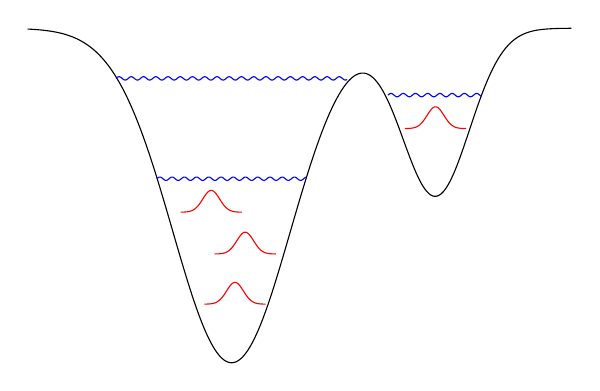
\begin{tikzpicture}
	\def\lims{xmin=-6,xmax=10,ymin=-2.1,ymax=0.01}
    \begin{axis}[\lims,hide x axis, hide y axis,width=0.7\textwidth,height=0.5\textwidth]
	    \addplot[mark=none,samples=1000,domain=-10:10,y domain=-2.1:0.01] {-2*exp(-x*x/6)-1*exp(-(x-6)*(x-6)/2)};
	    \addplot[red,mark=none,samples=1000,domain=-0.8:1.0] {-1.65+0.13*exp(-49*(x-0.1)*(x-0.1)/6)};
	    \addplot[red,mark=none,samples=1000,domain=-0.5:1.3] {-1.35+0.13*exp(-49*(x-0.4)*(x-0.4)/6)};
	    \addplot[red,mark=none,samples=1000,domain=-1.5:0.3] {-1.1+0.13*exp(-49*(x+0.6)*(x+0.6)/6)};
	    \addplot[blue,mark=none,samples=1000,domain=-2.2:2.2] {-0.9+0.01*sin(1000*(x+2.2))};
	    \addplot[blue,mark=none,samples=1000,domain=-3.4:3.4] {-0.3+0.01*sin(1000*(x+3.4))};
	    
	    \addplot[red,mark=none,samples=1000,domain=5.1:6.9] {-0.60+0.13*exp(-49*(x-6.0)*(x-6.0)/6)};
	    \addplot[blue,mark=none,samples=1000,domain=4.6:7.35] {-0.4+0.01*sin(1000*(x-4.6))};
	\end{axis}
	\end{tikzpicture}
	\caption{A schematic representation of metadynamics. The free energy well is gradually filled up with small Gaussians, and a transition is facilitated.}\label{Fig:ES:metadynamics}
\end{figure}

%\begin{figure}[htbp]
%	\centering
%	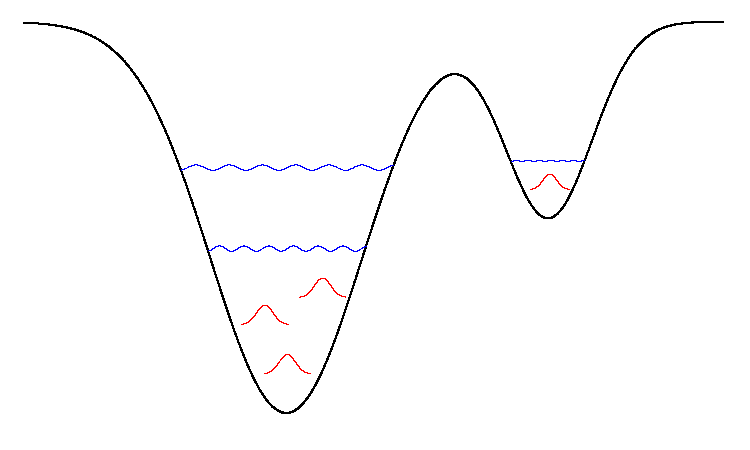
\includegraphics[width=0.8\textwidth]{figures/metadynamics.pdf}\\
%	\caption{A schematic representation of metadynamics. The free energy well is gradually filled up with small Gaussians, and a transition is facilitated.}\label{Fig:ES:metadynamics}
%\end{figure}

The above texts are merely an informal explanation of metadynamics. Formally, metadynamics belongs to a class of methods in which sampling is facilitated by introducing additional bias potential to pre-selected degrees of freedom, which are often referred as collective variables (CVs). In metadynamics, the bias potential added to the Hamiltonian of the system is history-dependent, and is often written as a sum of Gaussians deposited during the simulation as
\begin{equation}
   V_G(\mathbf{S},t) = \int\limits_0^tdt^\prime \omega\exp{\left(-\sum\limits_{i=1}^{d}\frac{\left[\mathbf{S}_i(R)-\mathbf{S}_i(R(t^\prime))\right]^2}{2\sigma_i^2}\right)}
\end{equation}
on a collective variable $\mathbf{S}$ in $d$-dimension. $\sigma$ and $\omega$ are two parameters tuning the shape of the Gaussians, which can be time-dependent. Asymptotically, 
\begin{equation}
   V_G(\mathbf{S},t\rightarrow \infty) = -G(\mathbf{S})+C.
\end{equation}

Metadynamics has been implemented in PLUMED (\url{https://plumed.github.io/doc-v2.3/user-doc/html/_metadyn.html}), which can work with major molecular dynamics packages.